\documentclass[a4paper]{article}

\usepackage{blindtext} % Package to generate dummy text throughout this template 

\usepackage[sc]{mathpazo} % Use the Palatino font
\usepackage[utf8]{inputenc}
\usepackage[T1]{fontenc} % Use 8-bit encoding that has 256 glyphs
\linespread{1.05} % Line spacing - Palatino needs more space between lines
\usepackage{microtype} % Slightly tweak font spacing for aesthetics

\usepackage[american]{babel} % Language hyphenation and typographical rules

\usepackage[hmarginratio=1:1,top=32mm]{geometry} % Document margins
\usepackage[hang, small,labelfont=bf,up,textfont=it,up]{caption} % Custom captions under/above floats in tables or figures
\usepackage{booktabs} % Horizontal rules in tables

\usepackage[backend=biber,style=ieee]{biblatex}
\usepackage{csquotes}
\bibliography{bibliography} 

\usepackage{mathtools}

\DeclarePairedDelimiter\abs{\lvert}{\rvert}

%%%%%%%%%%%%%%%%%%%%%%%%%%%%%%%%%%%%%%%%%%%%%%%%%%%%%%%%%%%%%%%%%%%%%%%%%%%%%%%
% Bilder
%%%%%%%%%%%%%%%%%%%%%%%%%%%%%%%%%%%%%%%%%%%%%%%%%%%%%%%%%%%%%%%%%%%%%%%%%%%%%%%
\usepackage{graphicx}
\usepackage{wrapfig}
\usepackage{float}
\graphicspath{{./resources/img/}}

%\usepackage{lettrine} % The lettrine is the first enlarged letter at the beginning of the text

\usepackage{enumitem} % Customized lists
\setlist[itemize]{noitemsep} % Make itemize lists more compact

%%%%%%%%%%%%%%%%%%%%%%%%%%%%%%%%%%%%%%%%%%%%%%%%%%%%%%%%%%%%%%%%%%%%%%%%%%%%%%%
% Listings
%%%%%%%%%%%%%%%%%%%%%%%%%%%%%%%%%%%%%%%%%%%%%%%%%%%%%%%%%%%%%%%%%%%%%%%%%%%%%%%
\usepackage{listings}

\usepackage[ruled, english]{algorithm2e}

\usepackage{xcolor}
\lstset{
	numbers=left,
	numberstyle=\tiny,
	numbersep=5pt,
	breaklines=true,
	showstringspaces=false,
	frame=single ,
	xleftmargin=15pt,
	xrightmargin=15pt,
	basicstyle=\ttfamily \footnotesize,
	stepnumber=2,
	captionpos=b,
	language=C,   %Sprache Festelegen
	floatplacement=H,
	tabsize=2,
	keepspaces=true
	%	keywordstyle=\color{blue},          % keyword style
	%	commentstyle=\color{dkgreen},       % comment style
	%	stringstyle=\color{mauve}         % string literal style
}


\lstdefinelanguage{scala}{
	morekeywords={abstract,case,catch,class,def,%
		do,else,extends,false,final,finally,%
		for,if,implicit,import,match,mixin,%
		new,null,object,override,package,%
		private,protected,requires,return,sealed,%
		super,this,throw,trait,true,try,%
		type,val,var,while,with,yield},
	otherkeywords={=>,<-,<\%,<:,>:,\#,@},
	sensitive=true,
	morecomment=[l]{//},
	morecomment=[n]{/*}{*/},
	morestring=[b]",
	morestring=[b]',
	morestring=[b]"""
}


\lstset{inputpath=./resources/code}


\usepackage{abstract} % Allows abstract customization
\renewcommand{\abstractnamefont}{\normalfont\bfseries} % Set the "Abstract" text to bold
\renewcommand{\abstracttextfont}{\normalfont\small\itshape} % Set the abstract itself to small italic text

\usepackage{titlesec} % Allows customization of titles
\titleformat{\section}[block]{\Large\scshape}{\thesection.}{1em}{} % Change the look of the section titles
\titleformat{\subsection}[block]{\large\scshape}{\thesubsection.}{1em}{} % Change the look of the section titles

\usepackage{fancyhdr} % Headers and footers
\pagestyle{fancy} % All pages have headers and footers
\fancyhead{} % Blank out the default header
\fancyfoot{} % Blank out the default footer
\fancyhead[C]{} % Custom header text
\fancyfoot[RO,LE]{\thepage} % Custom footer text

\usepackage{titling} % Customizing the title section

\usepackage[hidelinks]{hyperref} % For hyperlinks in the PDF
\usepackage{cleveref}

%----------------------------------------------------------------------------------------
%	TITLE SECTION
%----------------------------------------------------------------------------------------

\setlength{\droptitle}{-4\baselineskip} % Move the title up

\pretitle{\begin{center}\Huge\bfseries} % Article title formatting
	\posttitle{\end{center}} % Article title closing formatting
\title{An Architecture for Embedded Graphical Interfaces} % Article title

\author{%
	\textsc{Brendan Christy} \and \textsc{Ingo Braun} \and\\[-2ex]
	\vspace{1pt} \footnotesize Department of Computer Science, University of Applied Sciences RheinMain, Germany \\ 
	\vspace{1pt} \footnotesize \texttt{\{brendan.b.christy, ingo.braun\}@student.hs-rm.de}
}

\date{\today} % Leave empty to omit a date

\renewcommand{\maketitlehookd}{%
	\begin{abstract}
		\noindent With Project AEGIS we propose an open-source hardware based graphics accelerator for low-cost embedded systems, specifically for the VexRiscv by Charles Papon. 
		Like the VexRiscv, Project AEGIS will be written in SpinalHDL, a high level synthesis library for Scala, which simplifies 
		the process of creating your own hardware, as one can use the full featureset of Scala. During the project we will be able to
		rasterize lines and circles, bliting bit graphics, and will have a core for various arithmetic operations.
		The creation of an open-source hardware based graphics accelerator has several reasons. One key factor is to have hardware sovereignity, meaning to become independent form
		hardware manufacturers. Additionaly it is also important to learn how GPUs work, since not much of the inner workings is publicised. Lastly certain
		embedded systems have the need of displaying data. This can be done with Project AEGIS. TODO: REWRITE MOST OF IT
	\end{abstract}
}

%----------------------------------------------------------------------------------------
%TODO: Remove all PLACEHOLDERS
%TODO: Add REFERENCES
\begin{document}
	
	
	
	% Print the title
	\maketitle
	
	%----------------------------------------------------------------------------------------
	%	ARTICLE CONTENTS
	%----------------------------------------------------------------------------------------
	\section{Introduction}
	With the emergence of RISCV a need to become independent from hardware manufacturers has become clearer and clearer. This has lead to an open hardware movement. To support such a movement we have decided to create an open source hardware graphics accelerator. This means that we have to learn how old and modern GPUs work and how one could go and create a set of features that are necessary for drawing graphics on a screen. This graphics accelerator should run at a resolution of \(640 \times 480\), with the ability do draw lines, circles, font, sprites and fill rectangles.
	
	\section{Prerequisites}
	
	\subsection{GPU}
	\begin{itemize}
	\item Basic functionality of modern GPUs \cite{kilgariff2005geforce} have not changed over the years \cite{nvidia2018turing}
	\item Based on a graphics pipeline:
	\item Vertex Processing: Takes  three dimensional vertices and transforms it into screen space (what means screen space), each vertex independently
	\item Primitive Processing: Takes primitives, in this case a group of vertices that belong together and form a triangle, clips and culls them (what does that mean)
	\item Rasterization: Primitives are rasterized into so called pixel fragments (a group of undefined pixels without color information)
	\item Fragment processing: Afterwards these pixel fragments are then shaded to compute color at each pixel
	\item Pixel operation: Fragments are bleneded into the frame at their pixel locations (z-buffer determines visibility)
	\item as this is needed for each unit(vertex, primitive, fragment and pixel) independently, this is the of one core.
	\item A modern GPU can consist now at up to 2944 cores that all act in somewhat of the previously described functionality
\end{itemize}

	
	\subsection{Bresenham Algorithm}
	The original Bresenham Algorithms was developed by J. Bresenham in 1965~\cite{Bresenham65Line}. The target was to build a algorithm to draw a line between to coordinates on a pixel grid. The family of Bresenham Algorithms that exist, e.g. to draw a circle are developed by others. In the following section, the Bresenham Line and Circle algorithm will be explained.
\subsubsection*{Line Drawing}
The original line drawing algorithm uses only additions, subtractions, and a multiplication with the constant value of two. In a Cartesian coordinate system it exist eight variation of a gradient from a line, called octanes. The algorithm uses only one octants. It archived it by transforming the coordinates.

\begin{algorithm}[H]
	\SetAlgoLined
	\KwIn{\(x_0,~ y_0,~ x_1,~ y_1\)}
	\(\varDelta_x \gets \abs{x_1 - x_0}\)\;
	\(\varDelta_y \gets \abs{y_1 - y_0}\)\;
	\(\text{step}_x \gets x_0 < x_1~ ? ~1 ~:~ -1 \)\;
	\(\text{step}_y \gets y_0 < y_1~ ?~ 1 ~:~ -1\)\;
	err \( \gets \varDelta_x + \varDelta_y \)	
	\While{\(x_0 \neq x_1\) and \(y_0 \neq y_1\)}{
		draw Pixel at \(x_0 | y_0\) \;
		err2 \(\gets 2 \times err\)\;
		\If{err2 \(> \varDelta_y\)}{
			err \(\gets \text{err} + \varDelta_y\)\;
			\(x_0 \gets x_0 + \text{step}_x\)\;
		}
		\If{err2 \(< d_x\)}{
			err \(\gets \text{err} + \varDelta_x\)\;
			\(y_0 \gets y_0 + \text{step}_y\)\;
		}	
	}
	\caption{Bresenham Line Drawing Algorithm}
	\label{alg:bresline}
\end{algorithm}

The first step is to set the start coordinate. After that an error variable is set. The error variable is for the decision, which pixel is set next. Is value of the error variable smaller than zero it goes one step in the x direction, is the value bigger equal to zero it goes one step in the y and one step in the x direction. It ends when the new x and y coordinate equals the end x and y coordinate.
 
\subsubsection*{Circle Drawing}
The circle algorithm function are similar to the line algorithm but it has some differences. One difference is, that it has a circle radius and the coordinate of the middle point of the circle.
	
	\subsection{Bit Blit}
	\subsubsection*{Atari ST and Amiga Blitter} 
The functionality of a Bit Block Transfer Processor or Bit Blitter can be simply described as moving bit aligned data from a source to a destination with certain given logical operations. Not only could a Bit Blitter move sprites, but had an array of other features like filling an area with a given color or a pattern, transforming texts or rotating objects~\cite{atari1987blit}. Although its main purpose was a general memory-to-memory block copying.

Throughout the mid-1980s to the early 1990s several iterations of such a co-processor were created. The two major Bit Blitters known today were in the Atari ST and in the Commodore Amiga~\cite{data1988amiga}. Their basic functionality was virtually the same, they differentiated in one major aspect though. Their approach to moving data was different.

\subsubsection*{Moving Data}
In general terms the Bit Blit Processor took two memory blocks, usually a sprite and a mask~\cite{data1988amiga}. It combined them through a logical operation e.g a XOR, and the moved the result into the destination block.

The Atari STs approach for that type of operation was rather straight forward. It took as previously described, the result of the two sources with a logical operation and transferred it bit by bit. Meanwhile the Commodore Amiga took this design and expanded upon it~\cite{amigaBlitter}. It offered several modes of operation, among others a block mode and a line mode. Additionally the Amiga Blitter is does not operate on a bit level, but copies the data 16-bit word wise meaning it is a word Blitter.

Taken that into the account, if we have a screen with the resolution of \(320 \times 200\) with a total of 16 displayable colors and four bit-planes. The Amiga Blitter would have to do 20 operations per row on it as it consists of \(200\) rows of \(40\) bytes of data   


	
	\subsection{Advanced Extensible Interface   4 Bus}
	 
The  advanced microcontroller bus architecture (AMBA) advanced extensible interface 4 (AXI4) is a bus system specified by Advanced RISC Machines (ARM) in the year 2010 \cite{6129797}. The bus system has many features, thats why not all feature is described in detail in this chapter.

The AXI4 is a bus that can handle multiple master and slave over intermediate level called interconnect. This construction allows an n to n relation. The data bus width can be 32, 64, 128 and 256 bits. But the address bus is limited to 32 bits. Which means that he can only address 4 GB of memory space. For a high data transfer it can use the burst mode. With the burst mode, AXI4 can transfer 256 words without to align a new address. To establish and to release the communication it use a handshake protocol \cref{section:handshake}\cite{6129797}. 

\subsubsection{Handshake protocol}
\label{section:handshake}
This section describes the handshake protocol that is found in the AXI4 bus. The first step is that the master put on the address and when data are written the data. After that the master put an high signal on the valid signal

	
	\section{Design and Implementation}
	\subsection{VGA and Framebuffer}
	\subsubsection*{Design}\label{subsubsec:des_buff}
The needs for the implementation were clear from the start of the project. We knew that we are going to need some sort of output to a screen and a framebuffer for an image to be drawn to.

The design of the VGA interface was held flexible, as we wanted the option not only to exchange it with a different interface, but also that we are able to instantiate it with different resolutions. If the FPGA would allow it, a resolution of up to 1080p would be theoretically possible, as it generates its clock from a master clock that is fed in.

The framebuffer is designed to hold two frames at the same time, meaning it is a double buffer. This is something taken from GPU design, as this eliminates the chance of screen tear. This happens when one would want to draw into the image as it is being projected to the screen. Additionally the framebuffer should be instantiated with the maximal size of a frame and its depth of color.

To have the VGA interface and our graphics accelerator access it at the same time, we also decided to give it a true dual port design. As one of the ports is for the VGA interface to read from, while the other port is the the graphics accelerator to read from and write to.


\subsubsection*{Implementation}

As discussed in \cref{subsubsec:des_buff} the framebuffer will have two read ports an one write port. One read port is going to our core, which will be discussed in \cref{subsec:core}, and one is going to the VGA interface. To instantiate the buffer we need to pass it our configuration for the VGA interface. This can be found in the \texttt{VGAConfig} class. As seen in \cref{powtwo}, the calculation of the framebuffer size is done automatically. As it is more convenient to work with sizes that are of the power of two, we first have to increase it to the net number that is a power of two. Afterwards it creates its size by multiplying the horizontal and the vertical size and doubles it afterwards to create two buffers. 
\begin{lstlisting}[language=scala, caption={Resolution Check}, label=powtwo]
if (!isPow2(vAreaTemp)) {
	while(!isPow2(vAreaTemp)) {
		vAreaTemp = vAreaTemp + 1
	}
}

if (!isPow2(hAreaTemp)) {
	while(!isPow2(hAreaTemp)) {
		hAreaTemp = hAreaTemp + 1
	}
}

val bufferFrame = Mem(Vec(Bits(config.colorR bits), 
			  Bits(config.colorG bits), 
			  Bits(config.colorB bits)), 
			  2 * (vAreaTemp * hAreaTemp))
\end{lstlisting}
The VGA interface itself needs to generate a slow clock area with the frequency given in the VGAConfig. In this slow area is the implementation for the VGA interface, as it check that we are allowed to draw or are at the end of the line or the actual frame. The position of the current drawn pixel is held in a register. The information of which frame to read it gets from the framebuffer controller.

	
	\subsection{Bresenham Line and Circle}\label{subsec:des_bresenham}
	\subsubsection*{Design}

\subsubsection*{Implementation}
	
	\subsection{Bit Blit}
	\subsubsection*{Design}
As we want our bit blitter to be nothing more than the memory-to-memory blocking in the Atari ST. We are going to split this process up into two parts. One for the font drawing and one for the sprite drawing, as they have minor differences in how the data looks like.

Both of the will consist of eight by eight pixel information that has to be copied, the difference between them is that the font only consists of an alpha mask, the area which will be drawn, and one color for the letter to be drawn in. The sprite on the other hand has beside the alpha mask, the sprite data that needs to be drawn. This consists of an eight by eight grid of color information. 

\subsubsection*{Implementation}
A separate object is made to copy a letter from the font into the frame buffer. In its state machine we differentiate between the idle state and the copy state, seen in \cref{fontfsm}. When the idle state gets triggered it waits till the start flag is set, similar as in \cref{subsec:des_bresenham}. Once it is triggered to draw it sets a counter to zero and switches into the copy state.
\begin{lstlisting}[language=scala, caption={States of the Font Blitter}, label=fontfsm]
val idle = new State with EntryPoint
val copy = new State
\end{lstlisting}
In the copy state we evaluate each pixel of the alpha mask in a big switch-case. When the value of the pixel is set to high we write the color information for the corresponding pixel. When the whole alpha mask is done, for our case when the counter reaches 63, we go back into the idle state.
to know to which pixel to draw to, the first three bits act as a part of the x-coordinate and the last three bits count for y-coordinate.
\begin{lstlisting}[language=scala, caption={Copying the sprite color information into the frame buffer}, label={blitbuffer}]
for (i <- 4 to 67) {
	is(i) {
		vga.io.wData(0) := buffer(10 downto 0).resized
		vga.io.wData(1) := buffer(21 downto 11).resized
		vga.io.wData(2) := buffer(31 downto 12).resized
		vga.io.wAddress := (!switchVGA 
				  			## (storeVals1(1) + temp(5 downto 3)) 
				  			## (storeVals1(0) + temp(2 downto 0))).asUInt
		vga.io.wValid   := alpha(i - 4)
		counter := counter + 1
		valid := True
		goto(readRam)
	}
}
\end{lstlisting}
The sprite blitter is part of our core, which is discussed in \cref{subsec:core}. The way we have to copy the data functions similarly to how it is done in the font copying. We have to check if the alpha mask is set at a certain pixel. If it is we can draw the pixel of the sprite, this can be seen in \cref{blitbuffer}. Here we also use a switch-case to check the corresponding pixels.

	
	\subsection{AEGIS Core}
	\subsubsection*{Design}
As seen in \cref{img:coredes} the core will consist of a block of memory, an ALU combined with the blitter, and several smaller single function cores.

The graphic accelerator has a double frame buffer. It keeps track of the information of two separate frames. One of the frames is drawn by the VGA module, the other is being created by the graphics accelerator and CPU. The data for the objects are moved into the RAM of the CPU.

As some functions of the blitter correlate with the functions of the ALU (REFERENCE TO AMIGA MANUAL), the two blocks will be merged together in the following the two of them will be referred to as only the ALU. This part of the core will either write directly into the frame buffer or it will delegate the drawing to the proper function core. These smaller function cores consist of the basic graphical primitives, as discussed in \cref{subsec:des_bresenham}.
\begin{figure}[H]
	\centering
	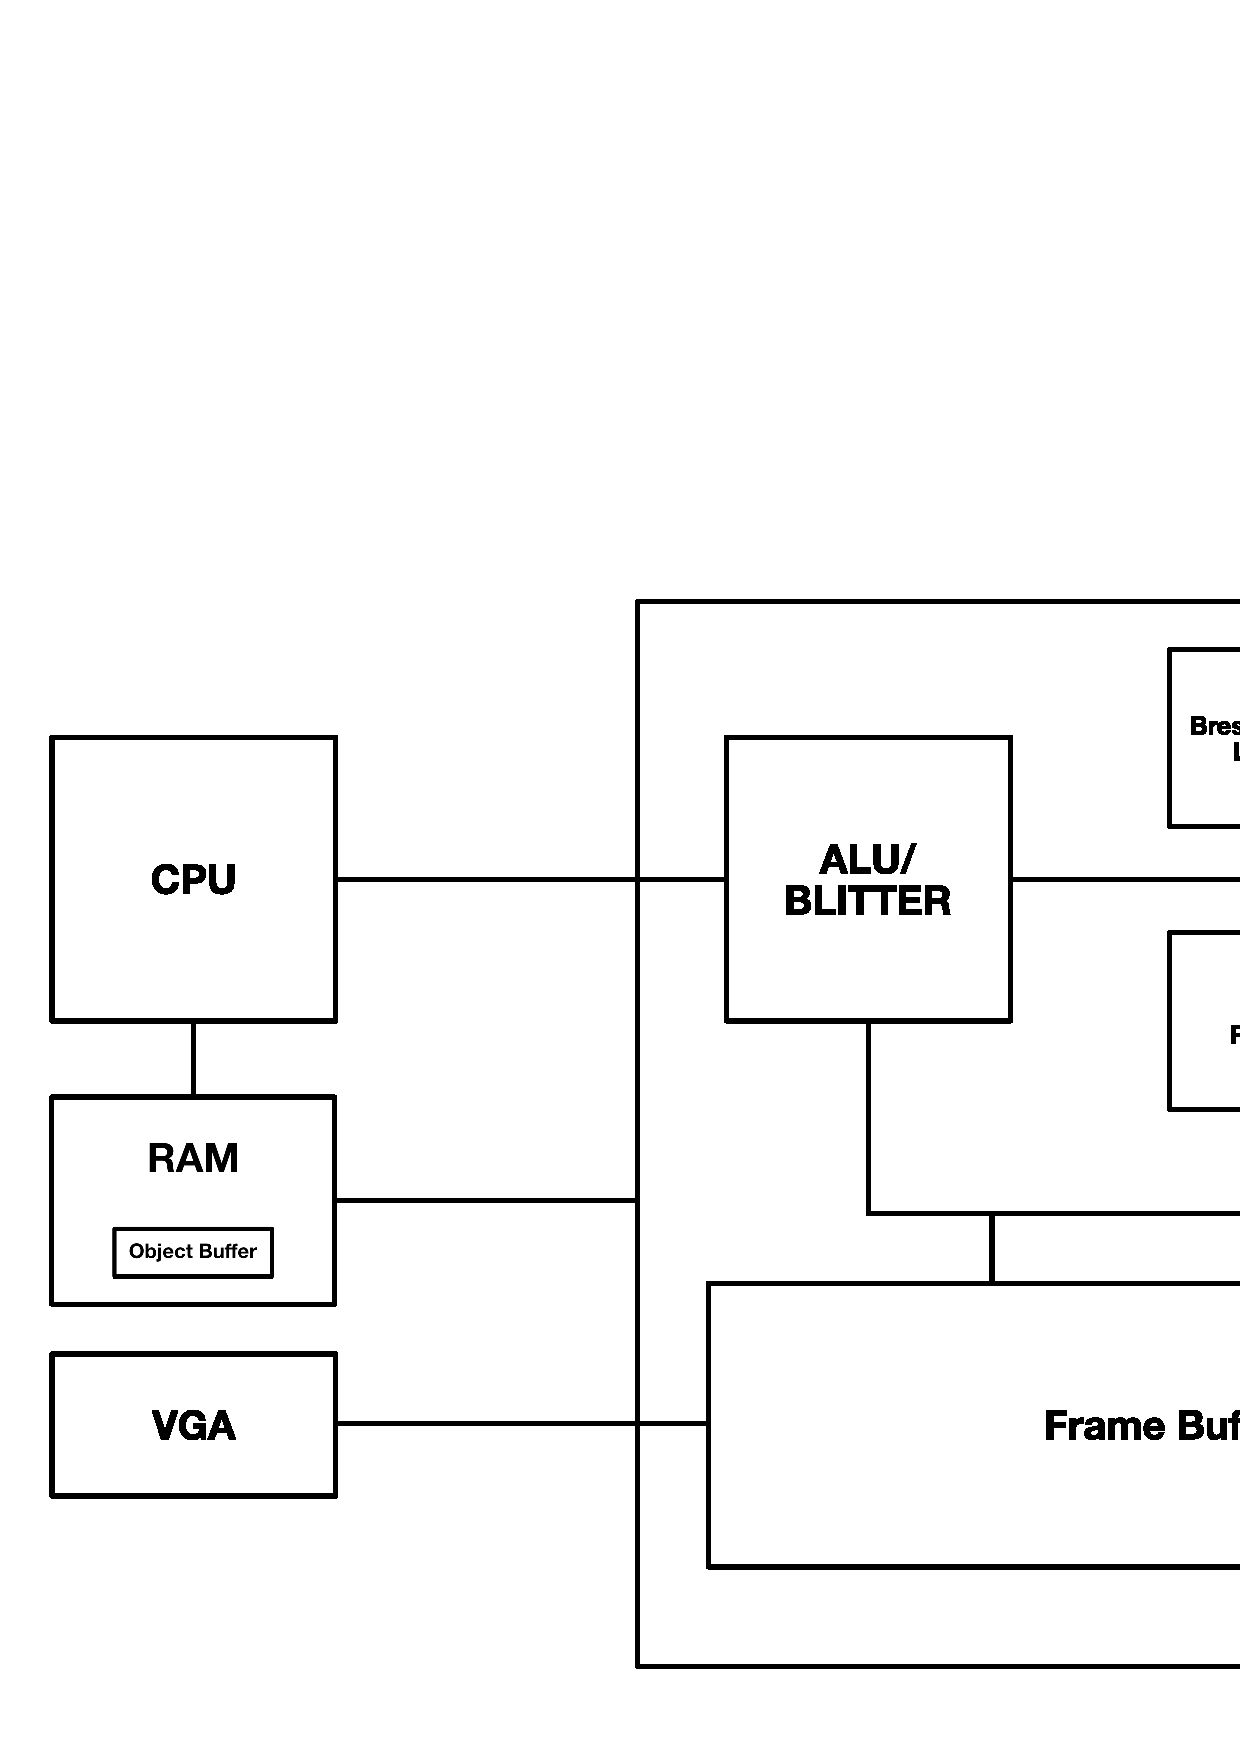
\includegraphics[width=0.5\textwidth]{coredesign}
	\caption{Graphical Design of the AEGIS Core }
	\label{img:coredes}
\end{figure}

For the communication between the CPU and the graphics accelerator, we use two AXI4 buses. The first one is a Axi4Shared for the communication with the CPU, and the second one is a Axi4readonly for the communication with the RAM.

When a write command is send over the AXI4 bus the graphics accelerator looks at the address. Is the address in the range of the double frame buffer, then it writes to it. Otherwise the address determines, what the graphics accelerator do. Further information he needs to operate get it from RAM at the address in the data value. 

\subsubsection*{Implementation}
\begin{itemize}
	\item is the main controll system, that is why is called mcp (tron)
	\item it has two state machine, the second one is a nested one
	\item it controlls both axi buses, the shared one as a slave and the readonly as a master
	\item the idle state waits until on the slave axi bus the following signal are set io.axicpu.sharedCmd.valid and he looks if the axi bus wants to read or write
	\item after that when the 25 bit is set it saves some data from the axi bus and goes to a wait state
	\item in the wait state it set the needed axi bus signals for the handshake and goes to the respones state
	\item here it set the neede signals for the responseand wait until the axi bus says its ok, after that it goes to the readdata state. or it goes to the switch state if a switch frame buffer is requested
	\item befor the switch case in the readdata is running, the nested state machine is activated
	\item the nested state machine is for the communication to the ram.
	\item it set the needed signals for the axi master bus, like how big is a word and the burst mode
	\item the read state is diveded in two stages the first one get the signals and the second one saves it into the temp variables
	\item the second state is divided into four states because we need different variables, and the sprite state saves the sprite directly to the framebuffer
	\item when all the data are read it goes to the exit state, we can have only one exitState int the hole state machine
	\item after the nested state machine is ready the readdata state determine which function we want
	\item after the function are ready it goes to the idle state.
	\item when the 23 bit is not set, the state machine read or write directly to the framebuffer. The programmer must keep track which framebuffer he want to read or write
\end{itemize}
	
	
	\section{Conclusion}
	With the results of this project, we have to ask ourselves several question:

\begin{description}
	\item[Did we achive everything planed for the Project?] Unfortunately we had to cut back on some features. We are only able to draw up to eight colors at a resolution of \(320 \times 240\). This is unfortunately the result of the lack of memory on the development boards. If the Altera development boards would have true dual port block memory, then we would have achieved a resolution of up to \(640 \times 480\).
	\item[What was easier than expected?] Two parts were simpler to implement than expected. The Bresenham algorithms fall under this category, as it was almost possible to implement them as they are in software. Also the implementation of the API went quicker than expected, with less errors than expected.
	\item[What was more difficult than expected?] The biggest problem that occurred during the implementation of the graphic accelerator, was the connection to the AXI bus. Not only was it difficult to understand the architecture itself, but also to understand how to use the implementation of the bus for SpinalHDL. This resulted in the most workload of the project.
	\item[Did the results line up with our expectations?] The final results of our project went far and beyond our expectations we had in the beginning of the project. We expected to achieve a frequency of around 45 MHz, which in the end got almost doubled. We also did not expect the difference in cycles needed. We expected more of a factor of between 20 and 30, but not a speedup of up to the factor of 160.
\end{description}


	
	\section{Future Work}
	for a maybe future work paralism (algorithms)
	
	\printbibliography
	
	
\end{document}